\documentclass[12pt, letterpaper]{article}
\usepackage{graphicx}
\graphicspath{{images/}} 
\usepackage{titling}
\usepackage{amsmath}
\usepackage{listings}
\usepackage{xcolor}
\usepackage{textcomp}
\usepackage{multicol}
\usepackage[utf8]{inputenc}
\usepackage{parallel}
\usepackage{siunitx}
\usepackage{booktabs}
\usepackage{fancyhdr}
\usepackage{tabularx}
\usepackage{caption}
\usepackage[export]{adjustbox}
\usepackage[top=1in, left=0.5in, right=0.5in, bottom=1in]{geometry}
\addtolength{\topmargin}{0in}

\usepackage{libertine}
\renewcommand*\familydefault{\sfdefault}  %% Only if the base font of the document is to be sans serif
\usepackage[T1]{fontenc}







\title{Spatial Mapping System Using Time-of-Flight}
\author{Hamza Siddiqui - 400407170 - siddih38 }
\date{April 17, 2023}

%\begin{document}

\pagestyle{fancy}

\lhead{Hamza Siddiqui}
%\chead {\today}
\chead {April 17, 2023}
\rhead{SMSUTOF HS 2023 v0.1}


\onecolumn

\begin{figure}
\begin{minipage}{0.47\textwidth}
\centering

\includegraphics[width=.7\textwidth,left,height=.4\textwidth]{logo.png}

\end{minipage}
\hfill
\begin{minipage}{0.47\textwidth}
\raggedleft
\Huge \textbf{Spatial Mapping System using ToF v0.1}
\end{minipage}
\end{figure}


\begin{figure}
\begin{minipage}{0.47\textwidth}

\section*{Core Device Components}
\begin{itemize}
    \item Microcontroller Unit (ARM\textregistered \ Cortex\textregistered-M4F TI MSP432E401Y SimpleLink\texttrademark) 
    \item Stepper Motor (28BYJ-48 Velleman\textregistered\ 5 VDC Stepper Motor with ULN2003 Driver Board)
    \item Time-of-Flight Sensor (ST FlightSense\texttrademark \ VL53L1X)
    \item Additional Push Button 
    \item Removable Sensor Mount (Hamza Electronics\texttrademark)
    \item Fiberboard Case (Hamza Electronics\texttrademark)
\end{itemize}



\end{minipage}
\hfill
\begin{minipage}{0.47\textwidth}
\centering
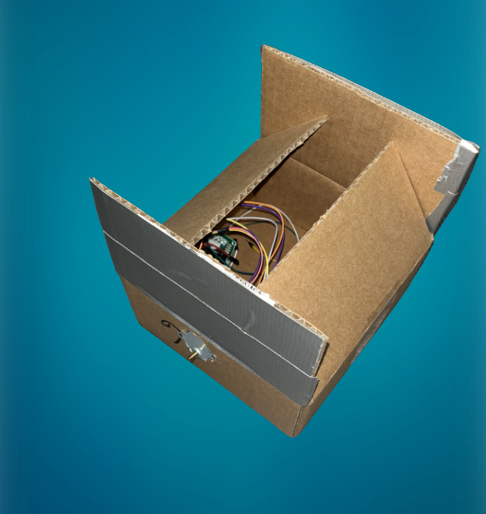
\includegraphics[width=0.7\textwidth,right]{image-removebg-preview (2).png} %PRODUCT IMAGE PLACEHOLDER

\end{minipage}
\end{figure}





\begin{document}
\maketitle
As a future member of the engineering profession, the student is responsible for performing the required work in an honest manner, without plagiarism and cheating.
Submitting this work with my name and student number is a statement and understanding that this work is my own and adheres to the Academic Integrity Policy of McMaster University and the Code of Conduct of the Professional Engineers of Ontario.
\thispagestyle{fancy}

\newpage
\section{Device Overview}
\subsection{Features}
\begin{multicols}{2}
\begin{itemize}
\item ARM Cortex-M4F TI MSP432E401Y Microcontroller (\$53.47)
    \begin{itemize}
        \item Bus frequency of 20MHz (configured via phase-locked loop; default core frequency of 120MHz)
        \item Four onboard LEDs - D3 flash functionality on each measurement
        \item Two onboard buttons (PJ1 for start/stop of motor rotation) and one reset button
        \item 1MB of flash, 256kB of SRAM
        \item  Communication interfaces including USB-OTG, CAN, Quad-SPI (QSSI), $\mathrm{I^2C}$, SPI,  and UART
        \item Two 12-Bit SAR-Based ADC Modules (2 Msps)
    \end{itemize}
\item MOT-28BYJ-48 Stepper Motor with ULN2003 driver (\$6.99)
    \begin{itemize}
        \item 5-12 VDC Operating Range 
        \item 64 steps/revolution 
        \item Frequency of 100Hz
        \item 4 phases with 4 step-indicator LEDs
    \end{itemize}
\item VL53L1X Time-of-Flight Sensor (\$25.32)
    \begin{itemize}
        \item Communication via $\mathrm{I^2C}$ (upto 400kHz)
        \item 4 m ranging and ranging frequency of 50Hz
        \item 2.6-5.5V supply range, 2.8V operating range
        \item Emitter: 940 nm invisible laser (Class1)
    \end{itemize}
\item Additional Push Button (\$0.60)
    \begin{itemize}
        \item Start/stop functionality for data acquisition
    \end{itemize}
\item Additional System Features
    \begin{itemize}
        \item UART serial communication between device and PC
        \item $\mathrm{I^2C}$ serial communication between device and Time-of-Flight sensor
        \item Baud rate of 115200
        \item C-language programming for device instructions, Python programming for visualization (via Pyserial and Open3d)
    \end{itemize}
\end{itemize}
\end{multicols}
\subsection{General Description}
To begin data acquisition, the additional push button is pressed to enable data processing, then the onboard button is pressed to begin taking measurements by spinning the motor and interfacing with the Time-of-Flight (ToF) sensor. The SMSUTOF HS 2023 utilizes a transducer which provides a digital output. Spatial distance measurements are acquired via the ToF sensor using $\mathrm{I^2C}$, while displacement is fixed at 30 cm. At each angle a measurement is taken, the D3 LED flashes. Together these measurements allow the device to measure a 3-D area. These signals are converted to electric signals, then conditioned into digital form and are finally converted to discrete digital values during the ADC process. The system communicates this to the user PC via UART asynchronous serial communication. A Python program is run on the PC and interfaces via their UART COM port and a baud rate of 115200, which then transfers measurement data to the PC and allows it to be stored in a .xyz file. This collected data is then used to generate a 3-D plot of the area that has been scanned via a Python program using open3d. The points for this plot are generated using trigonometric properties based on the angle and y,z coordinates generated, along with the fixed x-coordinate increment. If at anytime the button is pressed again during the scanning process, the data acquisition will be stopped. 
\subsection{Block Diagram (Data Flow Graph)}
\begin{figure}[h]
    \centering
    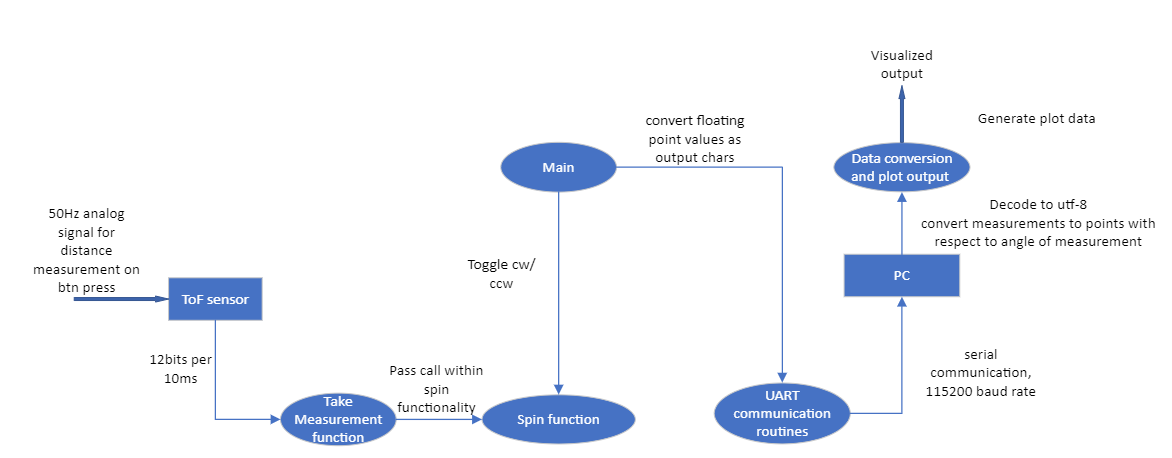
\includegraphics[width=\textwidth]{images/flowgraph.png}
    \caption{Flow graph}
    \label{fig:flowgraph}
\end{figure}

\section{Device Characteristics Table}
\begin{center}
\begin{tabularx}{0.5\textwidth}{|>{\centering\arraybackslash}X|>{\centering\arraybackslash}X|>{\centering\arraybackslash}X|}
\hline
\textbf{Characteristic} & \textbf{Description} \\
\hline
Bus Speed & 20MHz \\
\hline
Serial Port & COM4 \\
\hline
Communication Speed & 115200 bps \\
\hline
Measurement Status & D3 \\
\hline
\end{tabularx}
\captionof{table}{Device Characteristics}
\end{center}

\begin{minipage}{0.48\textwidth}
\centering
\textbf{Stepper Motor Pin Assignments}
\begin{tabular}{|c|c|}
\hline
\textbf{ULN2003 Driver Board} & \textbf{MCU} \\
\hline
+ (5V) & 5V \\
\hline
- (5V) & GND \\
\hline
IN1 & PH0 \\
\hline
IN2 & PH1 \\
\hline
IN3 & PH2 \\
\hline
IN4 & PH3 \\
\hline
\end{tabular}
\captionof{table}{Stepper Motor Pinout}
\end{minipage}
\hfill
\begin{minipage}{0.48\textwidth}
\centering
\textbf{Time-of-Flight Sensor Pin Assignments}
\begin{tabular}{|c|c|}
\hline
\textbf{VL53L1X} & \textbf{MCU} \\
\hline
VDD & - \\
\hline
VIN & VCC (3.3V or 5V) \\
\hline
GND & GND \\
\hline
SDA & PB3 (I2C0 SDA) \\
\hline
SCL & PB2 (I2C0 SCL)  \\
\hline
XSHUT & - \\
\hline
GPIO1 & - \\
\hline
\end{tabular}
\captionof{table}{Time-of-Flight Sensor Pinout}
\end{minipage}


\section{Detailed Description}
\subsection{Distance Measurement}\label{Distance Measurement}
\textbf{Acquisition:}\\
The VL53L1X sensor utilizes Light Detection and Ranging (LIDAR) technology to accurately measure distances. It emits a pulse of light with a wavelength of 940 nm, which is then reflected back to the sensor by an object (maximum 4 m away). The sensor measures the time it takes for the emitted light pulse to reach the object and be reflected back to the detector. By utilizing the known speed of light and the measured time, the VL53L1X calculates the distance to the object with high accuracy as follows:
$$Measured\ Distance = \frac{Photon\ Travel\ Time}{2}\times Speed\ of\ Light$$ The sensor is mounted to a motor that completes 360 degree rotations (512 steps). At every 64 steps, or 45 degrees, a user LED is flashed to indicate a measurement (in mm) has been taken by the sensor. This is achieved through interfacing with the sensor and micro controller via $\mathrm{I^2C}$ serial communication. In total, this allows for 8 measurements to be taken in a single rotation, and the program can be modified to measure at smaller number of steps to take more measurements for more accuracy at the cost of time (use-case dependent configuration). \\ 
\textbf{Data Processing:} \\
Data is processed and converted via mathematical computation. When given the motor's angle $\theta$, the program increments by the measurement angle rotation each time and computes the coordinates using trigonometric properties. This is computed as $angle = steps/(TOTAL STEPS) \times 2\pi$ where steps is incremented by 45 degrees and TOTAL STEPS is set to 512 - these reset each time a rotation is complete i.e. when 512 steps have completed. For a given distance measurement $r$, we obtain that $y = r\cos{\theta}$ and $z = r\sin{\theta}$ for the vertical plane. X coordinate is computed through configuring a physical step increment taken for each successive measurement rotation in the program and incrementing the coordinate for the next spatial scan based on this value (350mm default configuration). This is the displacement for each scan. Together these coordinates can be used for plotting and mapping. \\
\textbf{Example Calculation:} 
\begin{figure}[h]
    \centering
    \begin{minipage}{0.5\textwidth}
        Suppose a measurement $r$ is measured as 3 m at an angle of 45 degrees. Then,
        \begin{align*}
            y &= r\cos{45}\\
              &= 3\cos{45}\\
              &= 2.12132034356 \ \text{m}
        \end{align*}
        and 
        \begin{align*}
            z &= r\sin{45}\\
              &= 3\sin{45}\\
              &= 2.12132034356 \ \text{m}
        \end{align*}
    \end{minipage}%
    \begin{minipage}{0.5\textwidth}
        \centering
        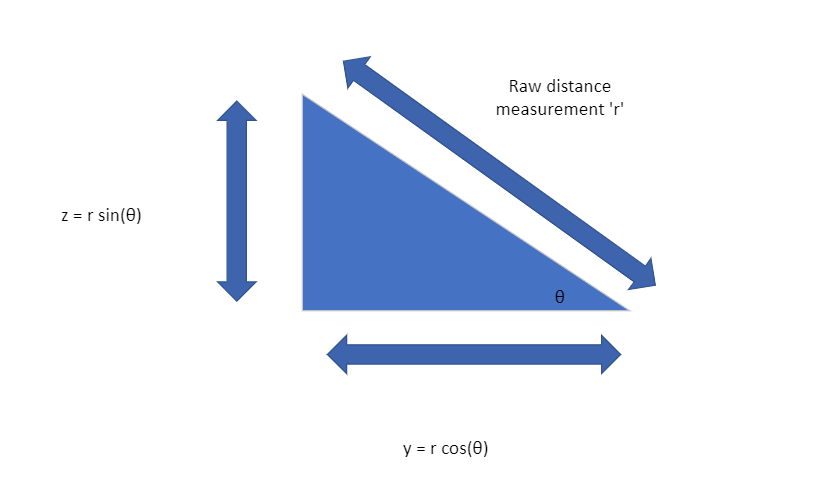
\includegraphics[width=\textwidth]{images/triangle.png}
    \end{minipage}
    \caption{Trigonometric Conversion: Solving for $y$ and $z$ using the sine and cosine functions.}
    \label{fig:trig_conversion}
\end{figure}

\subsection{Visualization}
The visualization is achieved through Python using the NumPy, open3d, and PySerial libraries. Data is communicated using UART and a specified PORT which is accessed via PySerial. The measurement data from the micro controller is then communicated to the PC and is processed as points following the previously outlined conversion method. The points are then written to a .xyz file in the format of "x y z" per line, and is outputted on the console in the same manner for the user to view measurements printed in real time for each measurement. Next, using open3d, the points are viewed numerically by conversion using NumPy. 
\\Here is an example of how to read a point cloud using the Open3D library:

{\fontsize{10pt}{12pt}\selectfont % set font size to 10pt with 12pt line spacing
    \ttfamily % switch to monospaced font
    \begin{verbatim}
        pcd = o3d.io.read_point_cloud("pointdata.xyz", format="xyz")

    \end{verbatim}
}
In this code snippet, the variable \verb|pcd| stores the point cloud data read from the file \verb|pointdata.xyz|. The \verb|format| parameter specifies the format of the file, which in this case is XYZ format. 
These are then visualized using the following function call:
{\fontsize{10pt}{12pt}\selectfont % set font size to 10pt with 12pt line spacing
    \ttfamily % switch to monospaced font
    \begin{verbatim}
    o3d.visualization.draw_geometries([pcd])
    \end{verbatim}
}
Next, each vertex from the data is appended and the coordinates to connect lines in each yz slice is defined. The lines are then mapped to the 3D coordinate vertices as a line set and are then outputted to the GUI for visualization with the following function calls:
{\fontsize{10pt}{12pt}\selectfont % set font size to 10pt with 12pt line spacing
    \ttfamily % switch to monospaced font
    \begin{verbatim}
    line_set = o3d.geometry.LineSet(
        points=o3d.utility.Vector3dVector(np.asarray(pcd.points)),
        lines=o3d.utility.Vector2iVector(lines)
    )

    o3d.visualization.draw_geometries([line_set])
    \end{verbatim}
}

In this code snippet, the \verb|LineSet| class is used to create a line set from a set of points and lines. The \verb|points| argument is a vector of 3D points, and the \verb|lines| argument is a vector of pairs of point indices that define the line segments. The resulting line set is then visualized using the \verb|draw_geometries| function from the Open3D visualization module.

\section{Application Example with Expected Output}

A spatial scan can be taken of a room with a set number of displacement increments. An example room with an expected output can be seen below:

\begin{figure}[htbp]
\centering
\begin{minipage}{0.48\textwidth}
\centering
\includegraphics[width=\linewidth]{hallway1.png}
\subcaption{Hallway POV 1}
\label{fig:hallway1}
\end{minipage}
\hfill
\begin{minipage}{0.48\textwidth}
\centering
\includegraphics[width=\linewidth, height = 0.75\textwidth]{hallway2.png}
\subcaption{Hallway POV 2}
\label{fig:hallway2}
\end{minipage}
\caption{Hallway scanned}
\label{fig:hallways}
\end{figure}

\begin{figure}[htbp]
\centering
\fbox{\begin{minipage}{0.48\textwidth}
\centering
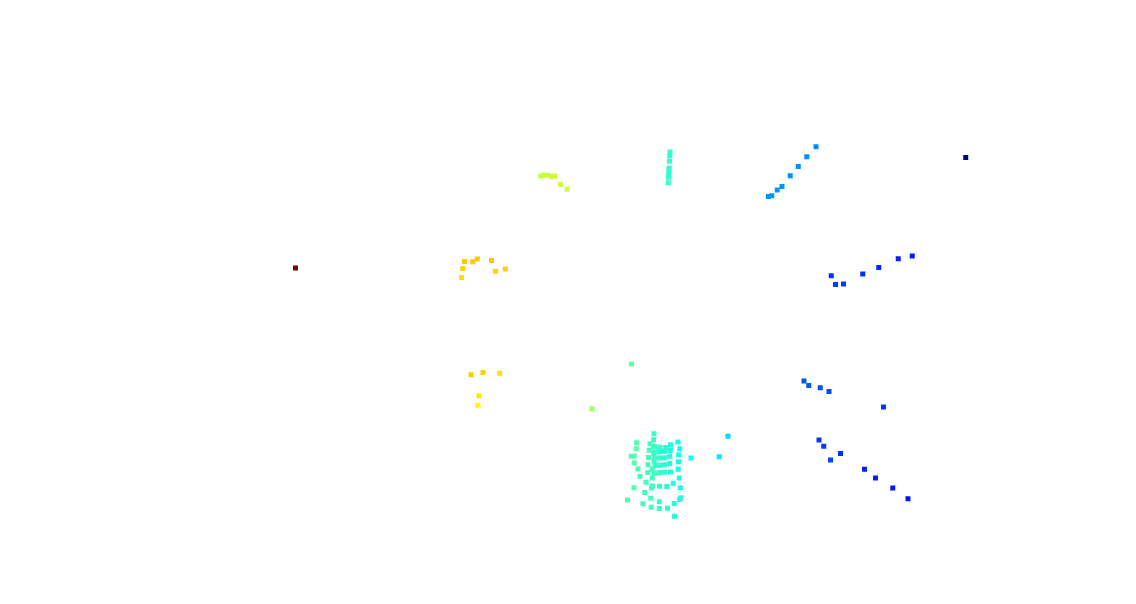
\includegraphics[width=\linewidth]{images/points.png}
\subcaption{Point Visualization}
\label{fig:points}
\end{minipage}}
\hfill
\fbox{\begin{minipage}{0.48\textwidth}
\centering
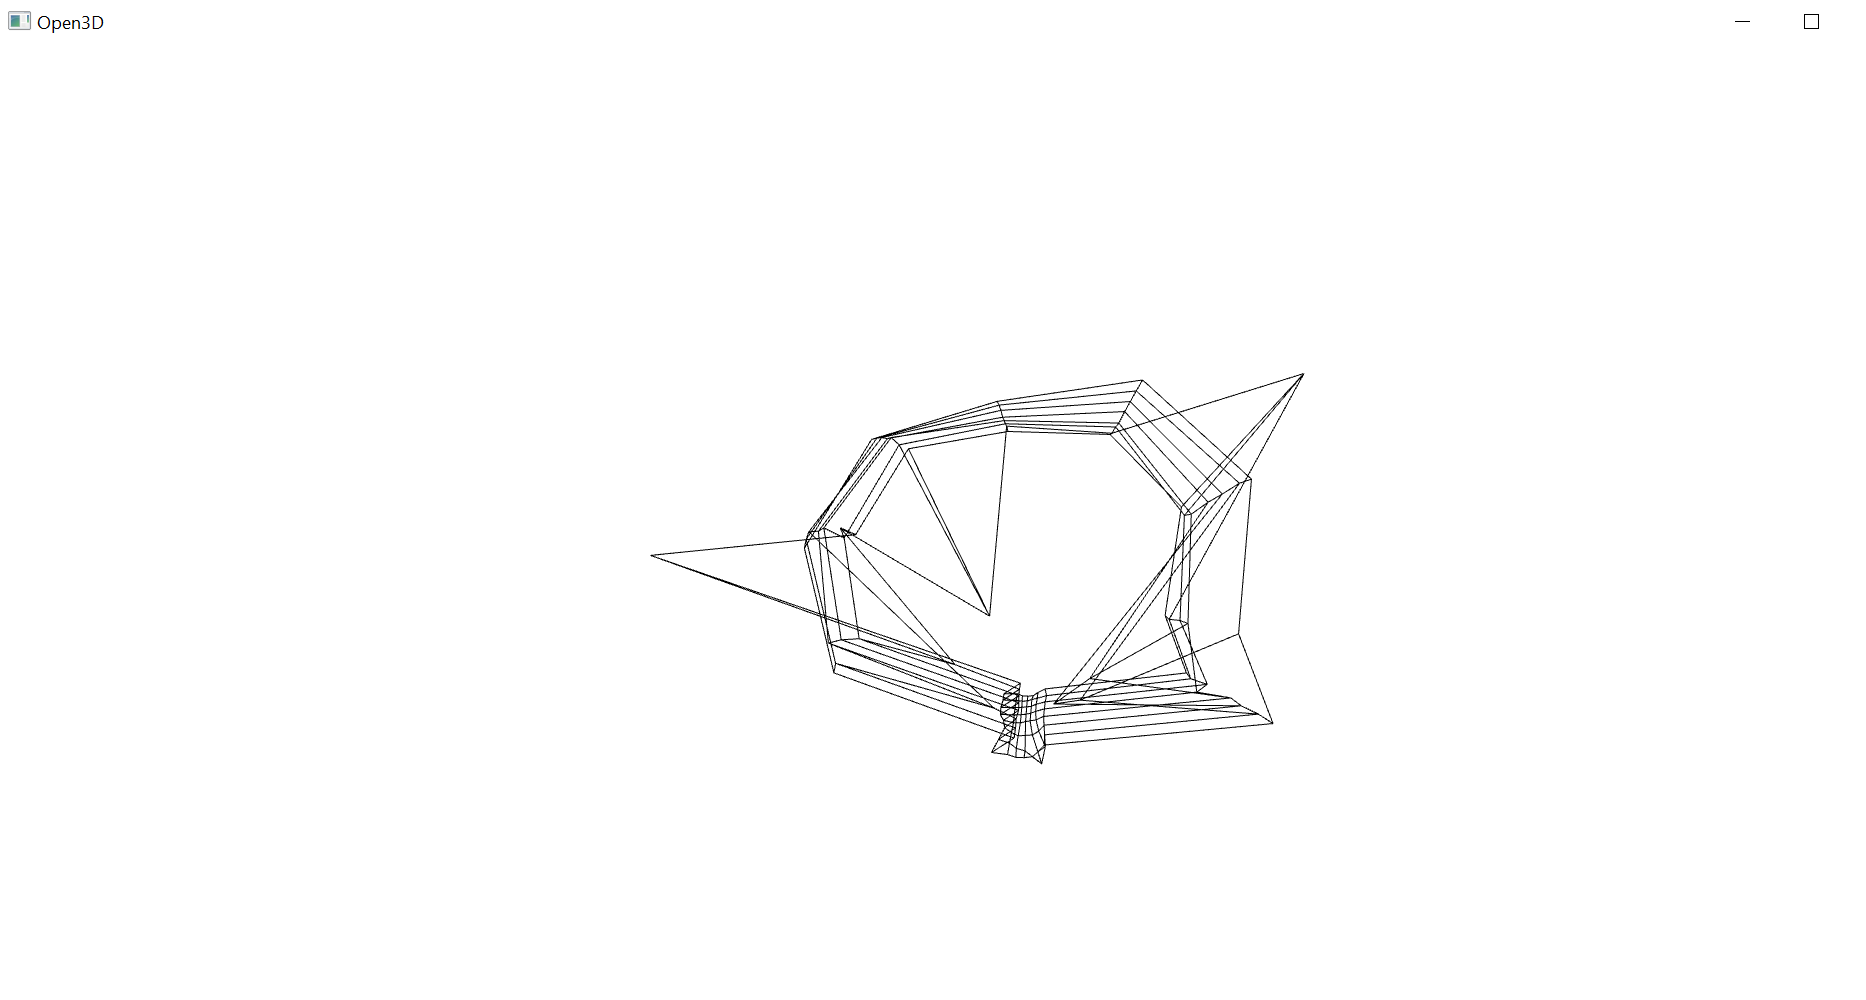
\includegraphics[width=\linewidth, height = 0.75\textwidth]{images/scan.png}
\subcaption{Final output spatial map}
\label{fig:scan}
\end{minipage}}
\caption{Expected output of scan}
\label{fig:scan}
\end{figure}
 \newpage
\section{User's Guide}
Setting up: \\
Build the circuit based on the schematic provided in section \ref{sec:Circuit Schematic}. Ensure the ToF is mounted to the stepper motor. The Keil project should be flashed on the micro controller by default, so pressing the reset button is sufficient to load the program. If this is not the case: Open the Keil Project src from the provided code and $Translate$ \rightarrow build \rightarrow load. \\

Software Installation:
\begin{enumerate}
    \item Download Python 3.9, which can be found at https://www.python.org/downloads/ under specific release downloads.
    \item Install NumPy, open3d, and Pyserial by opening terminal and typing:
\begin{verbatim}
pip install numpy
pip install open3d
pip install pyserial
\end{verbatim}
Refer to their documentation for any issues:
\begin{itemize}
\item NumPy documentation: \url{https://numpy.org/doc/1.21/}
\item Open3D documentation: \url{http://www.open3d.org/docs/release/}
\item Pyserial documentation: \url{https://pyserial.readthedocs.io/en/latest/pyserial.html}
\end{itemize}
\end{enumerate}

How to use the device after setting up: 
\begin{enumerate}
    \item Open \verb|measurement_data.py| and modify the PORT variable to that of your device, found from UART port listed in device manager. 
    \item Run \verb|measurement_data.py| by opening terminal, navigating to the directory of the file, and entering \verb|python measurement_data.py|
    \item Enter how many displacement steps the scan will use when prompted by the program. 
    \item Press the peripheral push button to enable measurements to set up the ToF. Pressing this again will toggle this back off.
    \item Press the the onboard PJ1 button each time a measurement rotation has to be made. Pressing this again will end the rotation process.
    \item For each number of physical steps taken, wait for the motor to complete one full rotation and return back to the home position. Once this is complete, move forward by the amount of x-displacement increment set (350 mm in the program but modifiable by user in the \verb|STEP_INCREMENT| variable) 
    \item Press the button again for the next measurement.
    \item The program will then print to you the measurements at each point taken as the program runs from the scan and also output this to a file in the same directory called \verb|pointdata.xyz|. D3 LED will flash on the micro controller for verification purposes. 
    \item Run the \verb|spatial_visualization.py| file by typing \verb|python spatial_visualization.py| in terminal.
    \item When prompted, enter the number of scans taken. The program will use this and then output the numerical value to the user in the console and output the visualization points on the screen in a GUI. Closing this screen will show a new screen with final spatial map in a GUI. 
\end{enumerate}
As explained earlier, the scan is of a yz plane with x being the displacement taken for each scan. y and z are seen as the vertical plane that the motor rotates and scans for, and x is the displacement after physically moving the motor by the step increment defined. Refer to section \ref{Distance Measurement} for more detailed information with example calculations.

\section{Limitations}
\begin{itemize}
    \item \textbf{FLoating Point Capability: }The micro controllers features a 120-MHz Arm® Cortex®-M4F Processor Core With Floating Point Unit (FPU). The FPU fully supports various single-precision operations such as add, subtract, multiply, divide, multiply-and-accumulate, and square root. It also provides conversions between fixed-point and floating-point data formats, and floating-point constant instructions. It has 32 dedicated 32-bit single-precision registers, which are also addressable as 16 double-word registers. With the limitation of bits, the computations communicated to the PC are given with truncation. The trigonometric computations done by Python's math library add to this as the infinite series are accurate to limits of double-precision floating-point arithmetic, 15 to 17 decimal digits. Together the accumulation of these truncations result in an imperfect calculation of points, however minimal. Furthermore the trignometric functions assume fixed angle inputs, which may be subject to error by upto a few degrees, hence the point is not computed at the exact angle the sensor was oriented at. This allows for the points to still be accurate to a certain reasonable precision without being entirely perfect. 
    \item \textbf{ToF Quantization Error: } The ToF module includes a quantization error in the ADC process. Quantization error is the difference between the analog signal and the closest available digital value at each sampling instant from the A/D converter. It is equivalent to resolution. It is computed using $m = 8$ from  the ADC module bits and $V_{FS} = 3.3\ \text{V}$.
    \begin{align*}
        resolution &= \frac{V_{FS}}{2^m} \\
                   &= \frac{3.3}{2^8} \\
                   &= 0.0129\ \text{V}
    \end{align*}
    \item \textbf{Serial Communication: } The maximum serial communication rate of the PC can be found from device manager and is seen as 128000 bps as seen in the UART port. The rate is limited when using the micro controller as the rate is capped at a baud rate of 115200 bps. This can be verified by interfacing with UART at different baud rates until receiving an error. An example can be seen below: 

\begin{figure}[htbp]
\centering
\begin{minipage}{0.48\textwidth}
\centering
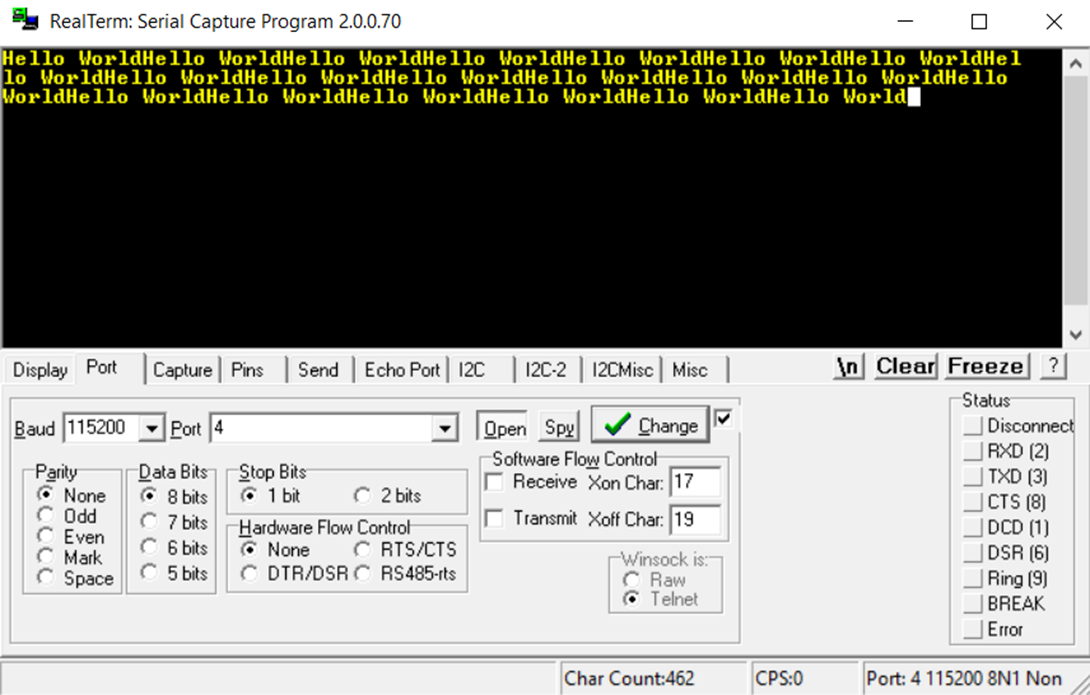
\includegraphics[width=\linewidth]{rt1.png}
\subcaption{RealTerm output at 115200 baud rate}
\label{fig:rt1}
\end{minipage}
\hfill
\begin{minipage}{0.48\textwidth}
\centering
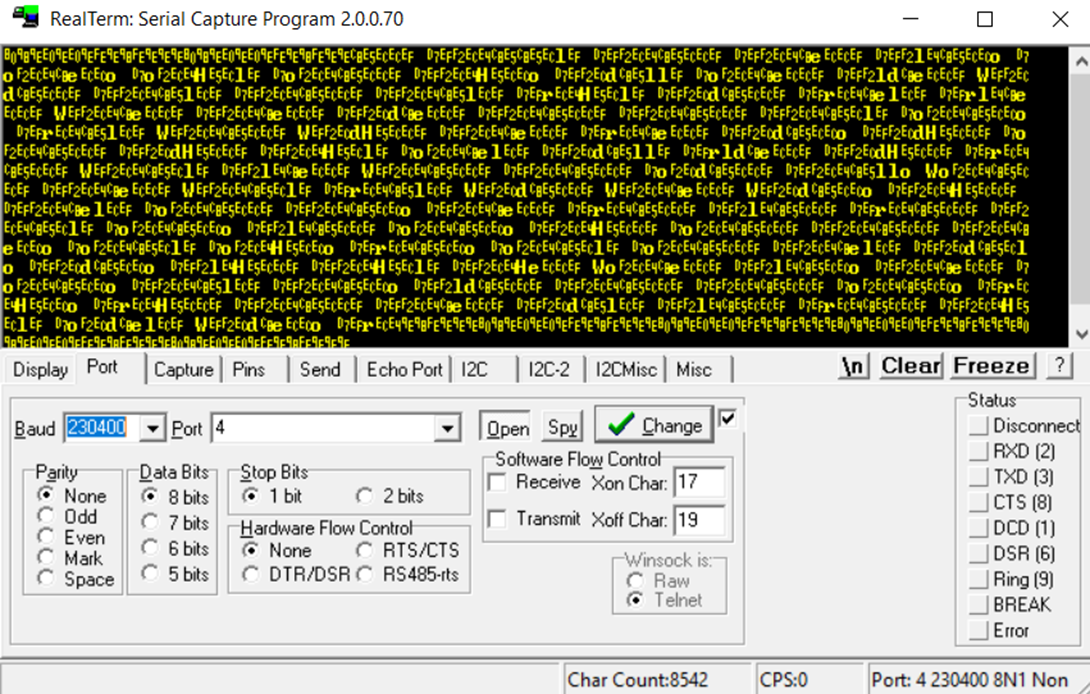
\includegraphics[width=\linewidth]{rt2.png}
\subcaption{RealTerm output above 115200 bps}
\label{fig:rt2}
\end{minipage}
\caption{Verification of maximum standard serial communication rate}
\label{fig:rt_verification}
\end{figure}
The microcontroller and time-of-flight modules communicate via I2C serial communication. The I2C ports on the microcontroller are configured with a 100 kbps clock (in standard mode), as specified in the datasheet. In this setup, the microcontroller assumes the role of leader while the time-of-flight sensor acts as the follower and operates based on the microcontroller's clock speed. 

\item \textbf{Speed Limitations: } The speed of the stepper motor is accounted for with 512 steps and delays using \verb|SystickWait(4000)| with a 20MHz bus speed. This gives a motor speed of 0.4096 s per rotation without measurement delays between. 
The ToF also had a speed limitation with a very quick default speed from the overall calculation formula mentioned, however the delays within the program outweigh this speed and become the limitation. The delay called was of 50ms. This was verified by toggling a GPIO output port before and after spinning, and before and after measuring, then visualizing this using oscilloscope probes from an Analog Discovery 2 board with a generated waveform, and visualizing the pulse generated for each. 
\end{itemize} 
\\
\section{Circuit Schematic}\label{sec:Circuit Schematic}

Below is the circuit schematic for the device:

\begin{figure}[htbp]
\centering
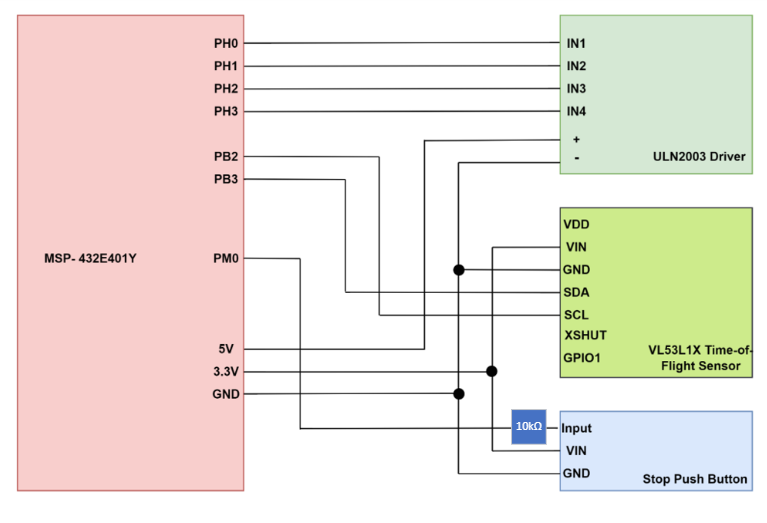
\includegraphics[width=0.8\textwidth]{schematic.png}
\caption{Circuit Schematic}
\end{figure}
\newpage
\section{Programming Logic Flowchart(s)}
Below is the programming logic flowchart of the system:
\begin{figure}[htbp]
\centering
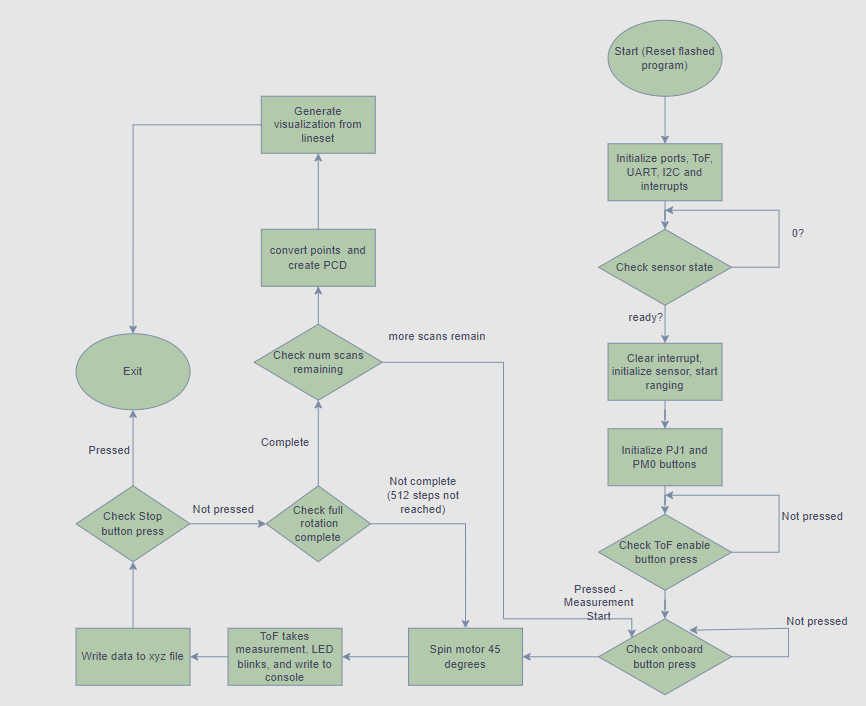
\includegraphics[width=0.8\textwidth]{images/chart.png}
\caption{Logic Flowchart}
\end{figure}
\newpage
\section{Additional Diagrams}
\begin{figure}[htbp]
\centering
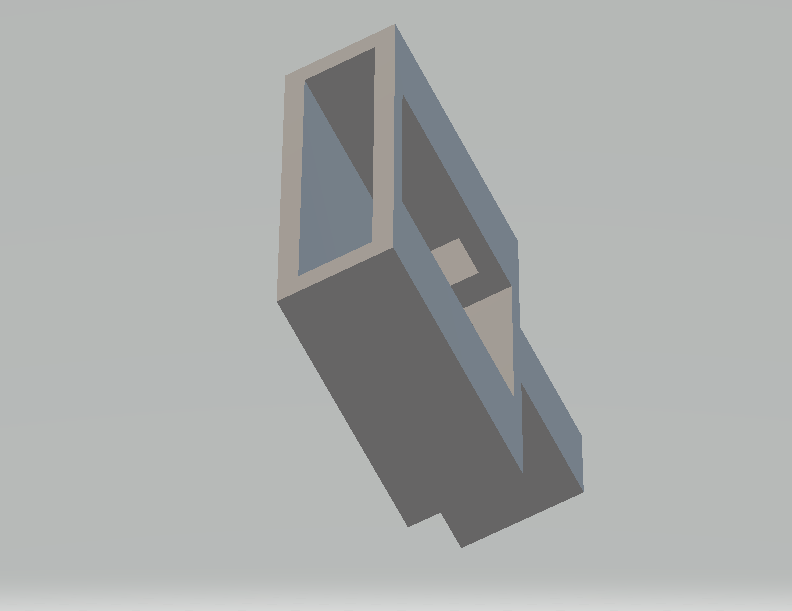
\includegraphics[width=0.8\textwidth]{images/mount.png}
\caption{ToF Mount STL}
\end{figure}
\end{document}